\documentclass[journal,12pt,onecolumn]{IEEEtran}
\usepackage{cite}
\usepackage{amsmath,amssymb,amsfonts,amsthm}
\usepackage{algorithmic}
\usepackage{graphicx}
\graphicspath{{./figs/}}
\usepackage{textcomp}
\usepackage{xcolor}
\usepackage{txfonts}
\usepackage{listings}
\usepackage{enumitem}
\usepackage{mathtools}
\usepackage{gensymb}
\usepackage{comment}
\usepackage{caption}
\usepackage[breaklinks=true]{hyperref}
\usepackage{tkz-euclide} 
\usepackage{listings}
\usepackage{gvv}                                           
\usepackage{xparse}
\usepackage{color}                                            
\usepackage{array}                                            
\usepackage{longtable}                                       
\usepackage{calc}                                             
\usepackage{multirow}
\usepackage{multicol}
\usepackage{hhline}                                           
\usepackage{ifthen}                                           
\usepackage{lscape}
\usepackage{tabularx}
\usepackage{array}
\usepackage{float}
\usepackage[margin=1in]{geometry}
\usepackage{fancyhdr}
\usepackage{chemfig}
\usepackage{multicol}
 \usepackage{amsmath}
\usepackage{enumitem}
\usepackage{array}
\usepackage{titlesec}
\usepackage{tabularx} 
\usepackage{amsmath, amssymb}
\usepackage{extarrows}
\usepackage{chemarr}
\usepackage[utf8]{inputenc}
\usepackage{chemmacros} 
\usepackage{graphicx}
\chemsetup{modules={reactions}} 
\begin{document}

\section*{\centering GA : GENERAL APTITUDE}

\noindent \textbf{1 -- 5 carry one mark each.}

\begin{enumerate}[label=\arabic*.]

\item Rajiv Gandhi Khel Ratna Award was conferred\_\_\_\_ Mary Kom, a six-time world champion in boxing, recently in a ceremony\_\_\_\_ the Rashtrapati Bhawan (the President’s official residence) in New Delhi.
\begin{multicols}{2}
\begin{enumerate}[label=(\Alph*)]
    \item with, at
    \item on, in
    \item on, at
    \item to, at
\end{enumerate}
\end{multicols}

\item Despite a string of poor performances, the chances of K. L. Rahul’s selection in the team are \_\_\_\_.
\begin{multicols}{2}
\begin{enumerate}[label=(\Alph*)]
    \item slim
    \item bright
    \item obvious
    \item uncertain
\end{enumerate}
\end{multicols}

\item Select the word that fits the analogy: \\ 
Cover : Uncover :: Associate : \_\_\_\_
\begin{multicols}{2}
\begin{enumerate}[label=(\Alph*)]
    \item Unassociate
    \item Inassociate
    \item Misassociate
    \item Dissociate
\end{enumerate}
\end{multicols}

\item Hit by floods, the kharif (summer sown) crops in various parts of the country have been affected. Officials believe that the loss in production of the kharif crops can be recovered in the output of the rabi (winter sown) crops so that the country can achieve its food-grain production target of 291 million tons in the crop year 2019-20 (July-June). They are hopeful that good rains in July-August will help the soil retain moisture for a longer period, helping winter sown crops such as wheat and pulses during the November-February period.\\

Which of the following statements can be inferred from the given passage?
\begin{enumerate}[label=(\Alph*)]
    \item Officials declared that the food-grain production target will be met due to good rains.
    \item Officials want the food-grain production target to be met by the November-February period.
    \item Officials feel that the food-grain production target cannot be met due to floods.
    \item Officials hope that the food-grain production target will be met due to a good rabi produce.
\end{enumerate}


\item The difference between the sum of the first $2n$ natural numbers and the sum of the first $n$ odd natural numbers is \_\_\_\_.
\begin{multicols}{2}
\begin{enumerate}[label=(\Alph*)]
    \item $n^2 - n$
    \item $n^2 + n$
    \item $2n^2 - n$
    \item $2n^2 + n$
\end{enumerate}
\end{multicols}

\end{enumerate}
\noindent \textbf{6 -- 10 carry two marks each.}

\begin{enumerate}[label=\arabic*.]
\setcounter{enumi}{5}

\item Repo rate is the rate at which Reserve Bank of India (RBI) lends commercial banks, and reverse repo rate is the rate at which RBI borrows money from commercial banks.\\

Which of the following statements can be inferred from the above passage?
\begin{enumerate}[label=(\Alph*)]
    \item Decrease in repo rate will increase cost of borrowing and decrease lending by commercial banks.
    \item Increase in repo rate will decrease cost of borrowing and increase lending by commercial banks.
    \item Increase in repo rate will decrease cost of borrowing and decrease lending by commercial banks.
    \item Decrease in repo rate will decrease cost of borrowing and increase lending by commercial banks.
\end{enumerate}

\item P, Q, R, S, T, U, V, and W are seated around a circular table.\\
I. S is seated opposite to W.\\
II. U is seated at the second place to the right of R.\\
III. T is seated at the third place to the left of R.\\
IV. V is a neighbour of S.\\

Which of the following must be true?
\begin{multicols}{2}
\begin{enumerate}[label=(\Alph*)]
    \item P is a neighbour of R.
    \item Q is a neighbour of R.
    \item P is not seated opposite to Q.
    \item R is the left neighbour of S.
\end{enumerate}
\end{multicols}

\item The distance between Delhi and Agra is 233 km. A car $P$ started travelling from Delhi to Agra and another car $Q$ started from Agra to Delhi along the same road 1 hour after the car $P$ started. The two cars crossed each other 75 minutes after the car $Q$ started. Both cars were travelling at constant speed. The speed of car $P$ was 10 km/hr more than the speed of car $Q$. How many kilometers the car $Q$ had travelled when the cars crossed each other?
\begin{multicols}{2}
\begin{enumerate}[label=(\Alph*)]
    \item 66.6
    \item 75.2
    \item 88.2
    \item 116.5
\end{enumerate}
\end{multicols}

\item For a matrix $M = [m_{ij}];~i,j=1,2,3,4$, the diagonal elements are all zero and $m_{ij} = -m_{ji}$. The minimum number of elements required to fully specify the matrix is\_\_\_\_.
\begin{multicols}{2}
\begin{enumerate}[label=(\Alph*)]
    \item 0
    \item 6
    \item 12
    \item 16
\end{enumerate}
\end{multicols}
\item The profit shares of two companies P and Q are shown in the figure. If the two companies have invested a fixed and equal amount every year, then the ratio of the total revenue of company P to the total revenue of company Q, during 2013--2018 is \_\_\_\_.

\begin{figure}[H]
\centering
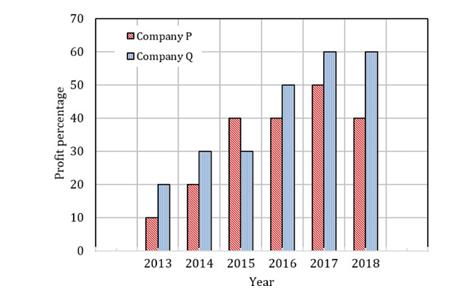
\includegraphics[width=0.7\columnwidth]{FIG/GA-10.png}
\caption*{}
\label{GA-10}
\end{figure}

\begin{multicols}{2}
\begin{enumerate}[label=(\Alph*)]
    \item 15 : 17
    \item 16 : 17
    \item 17 : 15
    \item 17 : 16
\end{enumerate}
\end{multicols}

\end{enumerate}
\newpage
\section*{\centering  P: Chemistry (Compulsory)}

\noindent \textbf{1 -- 5 carry one mark each.}

\begin{enumerate}[label=\arabic*.]

\item An aqueous solution contains a mixture of $10^{-8}$ M NaCl and $10^{-8}$ M HCl. Choose the correct statement about this solution.
\begin{enumerate}[label=(\Alph*)]
    \item The solution is a buffer with pH less than 7.00
    \item The solution is a buffer with pH greater than 7.00
    \item The solution is not a buffer but has its pH less than 7.00
    \item The solution is not a buffer but has its pH greater than 7.00
\end{enumerate}

\item The coordination complex which has a distorted octahedral structure is\\
(Given: Atomic numbers of V: 23; Mn: 25; Ni: 28; Cu: 29)
\begin{multicols}{2}
\begin{enumerate}[label=(\Alph*)]
    \item (Ni(H$_2$O)$_6$)$^{2+}$
    \item (Mn(H$_2$O)$_6$)$^{2+}$
    \item (V(H$_2$O)$_6$)$^{2+}$
    \item (Cu(H$_2$O)$_6$)$^{2+}$
\end{enumerate}
\end{multicols}

\item In naphthalene, the value of the integer "$n$" according to Hückel's rule of aromaticity is \_\_\_\_.

\item The azimuthal quantum number ($l$) of an electron in the d$_2$ orbital of a copper atom (atomic number: 29) is \_\_\_\_.

\item The standard enthalpy of reaction (in kJ mol$^{-1}$) for obtaining three moles of H$_2$(g) from atomic hydrogen in gas phase is \_\_\_\_.\\
(Given: Standard enthalpy of formation of atomic hydrogen in gas phase is 218 kJ mol$^{-1}$)

\end{enumerate}
\noindent \textbf{6 -- 11}

\begin{enumerate}[label=\arabic*., start=6]

\item The \textbf{correct} order of the first ionization energies of He, B, N and O in their corresponding ground state is
\begin{multicols}{2}
\begin{enumerate}[label=(\Alph*)]
\item He $>$ N $>$ O $>$ B
\item O $>$ N $>$ B $>$ He
\item He $>$ B $>$ N $>$ O
\item N $>$ O $>$ B $>$ He
\end{enumerate}
\end{multicols}

\item Based on the molecular orbital theory, which one of the following statements with respect to N$_2$, N$_2^+$, O$_2$ and O$_2^+$ is \textbf{correct}?
\begin{enumerate}[label=(\Alph*)]
\item Bond orders of N$_2$ and O$_2$ are higher than their corresponding cations.
\item Bond energy of N$_2^+$ is higher than that of N$_2$, whereas bond energy of O$_2^+$ is lower than that of O$_2$.
\item The unpaired electrons in N$_2^+$ and O$_2^+$ are present in $\sigma$ and $\pi^*$ orbitals, respectively.
\item The bond in N$_2^+$ is shorter than that in N$_2$, whereas bond in O$_2$ is shorter than that in O$_2^+$.
\end{enumerate}

\item Which one of the following statements is \textbf{incorrect} about the diborane molecule?
\begin{enumerate}[label=(\Alph*)]
\item B-H$^1$ bond is a 2-centre-2-electron bond (H$^1$: terminal hydrogen).
\item BH$^b$B bond is a 3-centre-2-electron bond (H$^b$: bridged hydrogen).
\item The bond angle H$^1$BH$^1$ is $122^\circ$ (H$^1$: terminal hydrogen).
\item The B-H$^1$ bond distance is longer than B-H$^b$ bond distance (H$^1$: terminal hydrogen, H$^b$: bridged hydrogen).
\end{enumerate}

\item Given below are Newman projections of ethylene glycol and 1,2-difluoroethane about their respective C--C bonds. The most stable conformations (lowest energy) of ethylene glycol and 1,2-difluoroethane are

\begin{figure}[H]
\centering
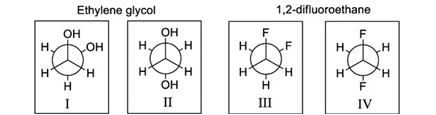
\includegraphics[width=0.7\columnwidth]{FIG/P-9.png}
\caption*{}
\label{GA-10}
\end{figure}

\begin{multicols}{1}
\begin{enumerate}[label=(\Alph*)]
\item I and III respectively.
\item I and IV respectively.
\item II and III respectively.
\item II and IV respectively.
\end{enumerate}
\end{multicols}

\item In the reaction given below, choose the condition that gives an anti-Markovnikov’s product.

\begin{figure}[H]
\centering
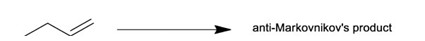
\includegraphics[width=0.7\columnwidth]{FIG/P-10.png}
\caption*{}
\label{P-10}
\end{figure}

\begin{multicols}{1}
\begin{enumerate}[label=(\Alph*)]
\item Peroxide / HCl
\item Aqueous mercuric acetate treatment
\item Diborane addition
\item Sulfuric acid addition
\end{enumerate}
\end{multicols}

\item Which one of the following hexoses will give an osazone that has a different melting point from that of the osazone obtained from D (+) glucose?
\begin{figure}[H]
\centering
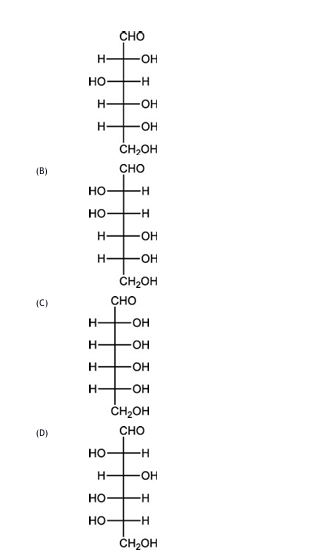
\includegraphics[width=0.7\columnwidth]{FIG/P-11.png}
\caption*{}
\label{P-11}
\end{figure}

\item A molecule in solution crystallizes into two different crystal forms with rate constants of 0.02~s$^{-1}$ and 0.13~s$^{-1}$. If the crystallization is assumed to be under kinetic control, then the half-life (in seconds, rounded off to one decimal place) of the molecule is \rule{3cm}{0.1pt}.


\item The standard potential ($E_\text{cell}^\circ$) for a cell reaction given below is +0.7~V. The standard reaction free energy ($\Delta_r G^\circ$) for this cell is \rule{3cm}{0.1pt}~kJ~mol$^{-1}$ (correct up to two decimal places). (Given: Faraday constant, F = 96500~C~mol$^{-1}$)\\
\text{Au$^{3+}$(aq) + 3 Ag(s) $\rightarrow$ Au(s) + 3 Ag$^+$(aq)}


\item The activation energy ($E_a$) estimated for a reaction from the Arrhenius equation is 21~kJ~mol$^{-1}$. If the frequency factor is assumed to be independent of temperature, then the ratio of the rate constants determined at 298~K and 260~K is \rule{3cm}{0.1pt} (rounded off to two decimal places). (Given: Gas constant, R = 8.315~J~K$^{-1}$~mol$^{-1}$)


\item At a given pressure, a substance is heated from 2000~K to 2600~K. If the entropy of the substance is 60~J~K$^{-1}$~mol$^{-1}$, and is assumed to be constant over the given temperature range, then the change in the chemical potential (in kJ~mol$^{-1}$) of the substance is \rule{3cm}{0.1pt}.

\end{enumerate}
\newpage
\section*{\centering  Q: Biochemistry}
\noindent \textbf{1 - 10 carry one mark each.}

\begin{enumerate}[label=\arabic*.]

\item Which one of the following hormones initiates a signaling cascade by directly binding to an intra-cellular receptor?
\begin{multicols}{2}
\begin{enumerate}[label=(\Alph*)]
    \item Insulin
    \item Gonadotropin
    \item Progesterone
    \item Epinephrine
\end{enumerate}
\end{multicols}

\item Which one of the following bonds is NOT present in ATP?
\begin{multicols}{2}
\begin{enumerate}[label=(\Alph*)]
    \item Phosphoester
    \item Phosphoanhydride
    \item N-Glycosidic
    \item $\alpha$-Glycosidic
\end{enumerate}
\end{multicols}

\item The reaction involved in the direct conversion of L-phenylalanine to L-tyrosine is
\begin{multicols}{2}
\begin{enumerate}[label=(\Alph*)]
    \item Hydroxylation
    \item Decarboxylation
    \item Transamination
    \item Reduction
\end{enumerate}
\end{multicols}

\item The human major histocompatibility complex (MHC) is
\begin{multicols}{2}
\begin{enumerate}[label=(\Alph*)]
    \item Polygenic and monomorphic
    \item Polygenic and polymorphic
    \item Monogenic and polymorphic
    \item Monogenic and monomorphic
\end{enumerate}
\end{multicols}

\item Har Gobind Khorana and Marshall Nirenberg elucidated the genetic code by using a cell-free protein synthesizing system. It was found that poly(U) and poly(C) result in the synthesis of poly(L-Phe) and poly(L-Pro), respectively. Based on these observations, which one of the following conclusions is correct?

\begin{enumerate}[label=(\Alph*)]
    \item Codon GGG specifies L-Phe and codon AAA specifies L-Pro
    \item Codon CCC specifies L-Phe and codon UUU specifies L-Pro
    \item Codon AAA specifies L-Phe and codon GGG specifies L-Pro
    \item Codon UUU specifies L-Phe and codon CCC specifies L-Pro
\end{enumerate}

\item Binding of an antibody to its cognate antigen does NOT involve
\begin{multicols}{2}
\begin{enumerate}[label=(\Alph*)]
    \item Covalent bonds
    \item Electrostatic forces
    \item Van der Waals forces
    \item Hydrogen bonds
\end{enumerate}
\end{multicols}

\item A globular protein of molecular weight 50 kDa exists as a mixture of monomers and dimers in solution. The most appropriate technique for the separation of these two forms of the protein is
\begin{multicols}{2}
\begin{enumerate}[label=(\Alph*)]
    \item Thin layer chromatography
    \item Ion exchange chromatography
    \item Gel filtration chromatography
    \item Paper chromatography
\end{enumerate}
\end{multicols}

\item Choose the correct order of molecules according to their ability to diffuse across a lipid bilayer.
\begin{multicols}{2}
\begin{enumerate}[label=(\Alph*)]
    \item CO$_2$ $>$ H$_2$O $>$ Glucose $>$ RNA
    \item CO$_2$ $>$ Glucose $>$ H$_2$O $>$ RNA
    \item RNA $>$ Glucose $>$ CO$_2$ $>$ H$_2$O
    \item H$_2$O $>$ CO$_2$ $>$ RNA $>$ Glucose
\end{enumerate}
\end{multicols}

\item When one glucose unit from glycogen gets converted to lactate in the muscle, the net number of ATP molecules produced is \rule{3cm}{0.1pt}.

\item Considering that the three pK$_a$s of histidine are pK$_1$=1.8, pK$_2$=9.2 and pK$_R$=6.0, its isoelectric point will be \rule{3cm}{0.1pt} (rounded off to one decimal place).
\noindent \textbf{11 - 20 carry two marks each.}
\item One mole of a native protein upon N-terminal analysis yielded one mole each of Asp and Val. Therefore, the protein in its native state exists as a
\begin{multicols}{2}
\begin{enumerate}[label=(\Alph*)]
    \item Monomer
    \item Homo-dimer
    \item Hetero-dimer
    \item Tetramer
\end{enumerate}
\end{multicols}

\item The prosthetic groups/cofactors involved in both 1e$^-$ and 2e$^-$ transfer in the mitochondrial electron transport chain are
\begin{multicols}{2}
\begin{enumerate}[label=(\Alph*)]
    \item NAD and NADP
    \item NAD and FAD
    \item Heme and FMN
    \item Coenzyme Q and FMN
\end{enumerate}
\end{multicols}

\item Match the items in \textbf{Group I} with the most appropriate items in \textbf{Group II} and choose the correct option.

\begin{center}
\begin{tabular}{|l|l|}
\hline
 Group I & Group II \\
\hline
P. Integrin & 1. Phagocytosis in the neural tissue \\
Q. Microglial cell & 2. Antigen processing by cross-presentation \\
R. TLR-7 & 3. Single stranded RNA recognition \\
S. Dendritic cell & 4. Binding of cells to endothelium \\
\hline
\end{tabular}
\end{center}

\begin{multicols}{2}
\begin{enumerate}[label=(\Alph*)]
    \item P-2, Q-1, R-3, S-4
    \item P-4, Q-1, R-3, S-2
    \item P-1, Q-2, R-3, S-4
    \item P-4, Q-1, R-2, S-3
\end{enumerate}
\end{multicols}

\item The correct combination of glycosidic linkages present in glycogen is
\begin{multicols}{2}
\begin{enumerate}[label=(\Alph*)]
    \item $\alpha$ 1$\rightarrow$4 and $\alpha$ 1$\rightarrow$6
\item $\alpha$ 1$\rightarrow$4 and $\beta$ 1$\rightarrow$6
    \item $\alpha$ 1$\rightarrow$6 and $\beta$ 1$\rightarrow$4
    \item $\alpha$ 1$\rightarrow$6 and $\beta$ 1$\rightarrow$6
\end{enumerate}
\end{multicols}

\item Polypeptides are either biosynthesized on the ribosomes using an mRNA template or chemically synthesized by the Merrifield’s solid phase method. The correct directions of peptide synthesis are
\begin{enumerate}[label=(\Alph*)]
    \item C$\rightarrow$N direction on the ribosomes and N$\rightarrow$C direction on the solid phase
    \item N$\rightarrow$C direction on the ribosomes and C$\rightarrow$N direction on the solid phase
    \item N$\rightarrow$C direction in both cases
    \item C$\rightarrow$N direction in both cases
\end{enumerate}

\item A solution absorbs 20\% of the incident light in a cuvette of path length 1.0 cm. The amount of light transmitted by the same solution in a cuvette of 3.0 cm path length is \rule{3cm}{0.1pt}\% (rounded off to one decimal place).

\item The second pK$_a$ of phosphoric acid is 6.8. The ratio of Na$_2$HPO$_4$ to NaH$_2$PO$_4$ required to obtain a buffer of pH 7.0 is \rule{3cm}{0.1pt} (rounded off to two decimal places).

\item A PCR in a 100~$\mu$L reaction volume, containing two primers at a concentration of 0.2~$\mu$M each, is set up to amplify a 250 base pair DNA fragment. Consider the average molecular weight of one base pair as 660~Da. If the primers are fully consumed by the end of the reaction, the amount of the final PCR product formed is \rule{3cm}{0.1pt}~$\mu$g (rounded off to one decimal place).

\item An enzyme obeying Michaelis-Menten kinetics shows a reaction velocity ($v$) of 10~$\mu$mol/min when the substrate concentration [S] equals its $K_\text{M}$. The maximal velocity $V_\text{max}$ for this enzyme is \rule{3cm}{0.1pt}~$\mu$mol/min (correct to integer number). ($K_\text{M}$ is Michaelis-Menten constant)

\item The enzyme glucose isomerase catalyzes the inter-conversion of glucose and fructose as shown.\\[0.2cm]
\textbf{Glucose $\rightleftharpoons$ Fructose}

The $\Delta G^\circ$ for this reaction is zero kcal/mol. After adding glucose isomerase to a 0.12~M glucose solution and allowing the reaction to attain equilibrium, the final concentration of fructose in the reaction mixture will be \rule{3cm}{0.1pt}~mM.


\end{enumerate}
\newpage
\section*{\centering  R: Botany}
\noindent \textbf{1 - 10 carry one mark each.}
\begin{enumerate}[label=\arabic*.]
\item Indefinite stamen is a characteristic feature of which of the following plant families?
\begin{multicols}{2}
\begin{enumerate}[label=(\Alph*)]
    \item Malvaceae
    \item Apocynaceae
    \item Poaceae
    \item Brassicaceae
\end{enumerate}
\end{multicols}

\item In natural condition, which of the following plants \textbf{DOES NOT} exhibit anomalous secondary growth?
\begin{multicols}{2}
\begin{enumerate}[label=(\Alph*)]
    \item Rice
    \item Aloe
    \item Yucca
    \item Dracaena
\end{enumerate}
\end{multicols}

\item In a typical angiosperm under natural condition, primary meristems are usually established during
\begin{multicols}{2}
\begin{enumerate}[label=(\Alph*)]
    \item Gametogenesis
    \item Embryogenesis
    \item Vegetative phase development
    \item Secondary growth
\end{enumerate}
\end{multicols}

\item 2-Methoxy-3, 6-dichlorobenzoic acid belongs to which class of plant growth regulators?
\begin{multicols}{2}
\begin{enumerate}[label=(\Alph*)]
    \item Synthetic auxin
    \item Synthetic cytokinin
    \item Strigolactone
    \item Brassinosteroid
\end{enumerate}
\end{multicols}

\item In a typical green plant, the first stable product of Calvin cycle is
\begin{multicols}{2}
\begin{enumerate}[label=(\Alph*)]
    \item Oxaloacetic acid
    \item Succinic acid
    \item Maleic acid
    \item 3-Phosphoglyceric acid
\end{enumerate}
\end{multicols}

\item Among the following, which best describes an organism that lives at the expense of other organisms, harmful but usually not killing?
\begin{multicols}{2}
\begin{enumerate}[label=(\Alph*)]
    \item Predator
    \item Symbiotic
    \item Prey
    \item Parasite
\end{enumerate}
\end{multicols}

\item The oleo-gum resin asafoetida (hing) is obtained from the cut surface of
\begin{multicols}{2}
\begin{enumerate}[label=(\Alph*)]
    \item Stem
    \item Root
    \item Leaf
    \item Fruit
\end{enumerate}
\end{multicols}

\item ‘Bakanae’ disease or ‘foolish seedling’ disease is caused by
\begin{multicols}{2}
\begin{enumerate}[label=(\Alph*)]
    \item Fungus
    \item Bacterium
    \item Virus
    \item Mycoplasma
\end{enumerate}
\end{multicols}

\item Which of the following chemicals is used for doubling of chromosome numbers during production of ‘doubled haploids’ in crop plants?
\begin{multicols}{2}
\begin{enumerate}[label=(\Alph*)]
    \item Hygromycin
    \item Kanamycin
    \item Colchicine
    \item Glufosinate
\end{enumerate}
\end{multicols}
\item An mRNA of a nuclear encoded plant gene, \textit{DSH20} has an ORF of 1353 nucleotides. Provided that average molecular weight of amino acid is 110 Dalton (Da), calculated molecular weight of DSH20 protein in kDa (\textit{round off to 1 decimal place}) is \rule{3cm}{0.1pt}.

\noindent \textbf{11 - 20 carry two marks each.}

\item \textbf{Group I, Group II and Group III} represent enzyme, product of the enzymatic reaction, and metabolic process, respectively.

\begin{center}
\begin{tabular}{|l|l|l|}
\hline
Group I & Group II & Group III \\
\hline
P. Hexokinase      & i. Malate             & 1. Glycolysis \\
Q. Fumarase        & ii. Glucose 6-P       & 2. Photorespiration \\
R. PEP Carboxylase & iii. Hydrogen peroxide & 3. TCA cycle \\
S. Glycolate oxidase & iv. Cinnamic acid    & 4. Photosynthesis \\
                   & v. Oxaloacetic acid   & \\
\hline
\end{tabular}
\end{center}

The \textbf{CORRECT} combination for Group I, Group II and Group III is
\begin{multicols}{2}
\begin{enumerate}[label=(\Alph*)]
    \item P-ii-1, Q-iv-3, R-v-2, S-iii-4
    \item P-ii-1, Q-i-3, R-v-4, S-iii-2
    \item P-ii-2, Q-v-3, R-i-4, S-iii-1
    \item P-iii-1, Q-i-3, R-iv-4, S-ii-2
\end{enumerate}
\end{multicols}

\item Match the following in \textbf{CORRECT} combination between Group I and Group II with reference to the agents that interfere with oxidative phosphorylation.

\begin{center}
\begin{tabular}{|l|l|}
\hline
Group I & Group II \\
\hline
P. Cyanide        & i. Blocks electron transfer from cyt b to cyt c$_1$ \\
Q. Antimycin A    & ii. Inhibits F$_1$ \\
R. Aurovertin     & iii. Uncoupling of phosphorylation from electron transfer \\
S. 2,4-Dinitrophenol & iv. Inhibits cytochrome oxidase \\
                  & v. Inhibits K$^+$ ionophore \\
\hline
\end{tabular}
\end{center}

\begin{multicols}{2}
\begin{enumerate}[label=(\Alph*)]
    \item P-iv, Q-i, R-ii, S-iii
    \item P-v, Q-i, R-iii, S-iv
    \item P-iv, Q-iii, R-ii, S-v
    \item P-v, Q-ii, R-iii, S-iv
\end{enumerate}
\end{multicols}
\item In relation to Agrobacterium mediated genetic engineering in plants, match the following in CORRECT combination.

Gene name \hspace{3cm} Function

P. virA \hspace{2.5cm} i. Acetosyringone receptor

Q. virB \hspace{2.5cm} ii. Conjugal tube formation

R. virD1 \hspace{2.3cm} iii. Topoisomerase

S. virG \hspace{2.7cm} iv. Inducer of all vir operons

\hspace{4.2cm} v. Octopine synthesis

\begin{multicols}{2}
\begin{enumerate}[label=(\Alph*)]
    \item P-iv, Q-iii, R-ii, S-v
    \item P-ii, Q-i, R-iii, S-v
    \item P-i, Q-ii, R-iii, S-iv
    \item P-iii, Q-i, R-ii, S-iv
\end{enumerate}
\end{multicols}

\item Match the plant part (Group I) with the product obtained (Group II) and the representative plant species (Group III) in CORRECT combination.
\newpage
\noindent
\begin{tabular}{|l|l|l|}
\hline
\textbf{Group I} & \textbf{Group II} & \textbf{Group III} \\
\hline
P. Bark   & i. Tannins        & 1. Papaver somniferum \\
Q. Leaf   & ii. Saffron       & 2. Camellia sinensis \\
R. Flower & iii. Codeine      & 3. Cinnamomum zeylanicum \\
S. Fruit  & iv. Aromatic oil  & 4. Crocus sativus \\
\hline
\end{tabular}
\begin{multicols}{2}
\begin{enumerate}[label=(\Alph*)]
    \item P-ii-1, Q-i-3, R-iv-2, S-iii-4
    \item P-ii-1, Q-i-2, R-iv-4, S-iii-3
    \item P-ii-2, Q-iv-3, R-i-4, S-iii-1
    \item P-iv-3, Q-i-2, R-ii-4, S-iii-1
\end{enumerate}
\end{multicols}

\item Select the CORRECT combination by matching the disease, causal organism and the affected plant.

\noindent
\begin{tabular}{|l|l|l|}
\hline
\textbf{Group I} & \textbf{Group II} & \textbf{Group III} \\
\hline
P. Bark   & i. Tannins        & 1. Papaver somniferum \\
Q. Leaf   & ii. Saffron       & 2. Camellia sinensis \\
R. Flower & iii. Codeine      & 3. Cinnamomum zeylanicum \\
S. Fruit  & iv. Aromatic oil  & 4. Crocus sativus \\
\hline
\end{tabular}
\begin{multicols}{2}
\begin{enumerate}[label=(\Alph*)]
    \item P-iv-1, Q-iii-3, R-i-2, S-ii-4
    \item P-ii-1, Q-i-6, R-iv-4, S-iii-2
    \item P-iii-1, Q-iv-3, R-i-5, S-ii-4
    \item P-iv-1, Q-ii-3, R-iii-2, S-i-5
\end{enumerate}
\end{multicols}

\item Match the following alkaloids with their uses and source plants in CORRECT combination.

\begin{tabular}{|l|l|l|}
\hline
Alkaloid      & Use                     & Source plant \\
\hline
P. Morphine   & i. Anti-cancer          & 1. Cinchona officinalis \\
Q. Quinine    & ii. Analgesic           & 2. Catharanthus roseus \\
R. Atropine   & iii. Anti-cholinergic   & 3. Papaver somniferum \\
S. Vinblastine & iv. Anti-malarial      & 4. Hyoscyamus niger \\
\hline
\end{tabular}
\begin{multicols}{2}
\begin{enumerate}[label=(\Alph*)]
    \item P-ii-3, Q-iv-1, R-iii-4, S-i-2
    \item P-ii-1, Q-i-3, R-iv-4, S-iii-2
    \item P-ii-2, Q-iv-1, R-i-4, S-iii-3
    \item P-iii-4, Q-ii-1, R-iv-3, S-i-2
\end{enumerate}
\end{multicols}
\item Match the following ecological terms with their appropriate definitions.

\begin{tabular}{|l|l|}
\hline
Term             & Definition \\
\hline
P. Niche         & i. Position of a species in food chain \\
Q. Biotas        & ii. Place of a living organism in the biotic environment and its relations to food and enemies \\
R. Trophic level & iii. Physical environment of an organism \\
S. Habitat       & iv. Totality of organisms (flora and fauna) in a given place or region \\
\hline
\end{tabular}
\begin{multicols}{2}
\begin{enumerate}[label=(\Alph*)]
    \item P-i, Q-ii, R-iv, S-iii
    \item P-ii, Q-iv, R-i, S-iii
    \item P-iv, Q-iii, R-i, S-ii
    \item P-iii, Q-ii, R-ii, S-iv
\end{enumerate}
\end{multicols}
\item Arrange the following ‘water reservoirs of earth’ in decreasing order of water volume.\\
P- Streams \quad Q- Groundwater \quad R- Glaciers \quad S- Lakes and inland seas
\begin{multicols}{2}
\begin{enumerate}[label=(\Alph*)]
    \item R-Q-S-P
    \item P-Q-R-S
    \item S-P-R-Q
    \item R-P-Q-S
\end{enumerate}
\end{multicols}
\item Selection markers and the corresponding genes used in plant genetic engineering are given below:

\begin{table}[h!]
\centering
\begin{tabular}{ll}
\textbf{Selection Marker} & \textbf{Gene} \\
P. Kanamycin & i. \textit{hptIV} \\
Q. Hygromycin & ii. \textit{bar} \\
R. Bialaphos & iii. \textit{pmi} \\
S. Mannose & iv. \textit{nptII} \\
\end{tabular}
\end{table}


Choose the \textbf{CORRECT} combination
\begin{enumerate}[label=(\Alph*)]
\item P-ii, Q-i, R-iv, S-iii
\item P-iv, Q-ii, R-i, S-iii
\item P-iv, Q-i, R-ii, S-iii
\item P-iii, Q-iv, R-ii, S-i
\end{enumerate}

\item A double homozygous mutant develops green and wrinkled seeds. When it was crossed with a true-breeding plant having yellow and round seeds, all the F1 plants developed yellow and round seeds. After self-fertilization of F1, the calculated percentage probability of plants with green and wrinkled seeds in the F2 population (\textit{rounded off to 2 decimal places}) is \rule{3cm}{0.1pt}.

\end{enumerate}
\newpage
\section*{\centering S : MICROBIOLOGY}

\noindent \textbf{1 -- 10 carry one mark each.}

\begin{enumerate}[label=\arabic*.]

\item The technique of microbial ``pure culture'' was pioneered by
\begin{multicols}{4}
\begin{enumerate}[label=(\Alph*)]
\item Edward Jenner
\item Louis Pasteur
\item Robert Hooke
\item Robert Koch
\end{enumerate}
\end{multicols}

\item The antibacterial trimethoprim is an inhibitor of
\begin{multicols}{2}
\begin{enumerate}[label=(\Alph*)]
\item dihydrofolate reductase
\item dihydropteroate synthase
\item N5,N10-methenyl tetrahydrofolate synthetase
\item serine hydroxymethyl transferase
\end{enumerate}
\end{multicols}

\item Choose the correct taxonomical hierarchy among the following:
\begin{enumerate}[label=(\Alph*)]
\item Species, Genus, Family, Order, Class, Phylum, Domain
\item Species, Genus, Order, Class, Family, Phylum, Domain
\item Species, Genus, Order, Family, Class, Phylum, Domain
\item Species, Genus, Family, Class, Order, Phylum, Domain
\end{enumerate}

\item Shifting a \textit{Saccharomyces cerevisiae} culture from fermentative to aerobic respiratory mode will
\begin{enumerate}[label=(\Alph*)]
\item decrease carbon dioxide production
\item increase alcohol production
\item increase glucose consumption
\item decrease ATP generation per mole of glucose
\end{enumerate}

\item Which one of the following diseases is treated by a neuraminidase inhibitor?
\begin{multicols}{2}
\begin{enumerate}[label=(\Alph*)]
\item Chickenpox
\item Polio
\item Influenza
\item Japanese encephalitis
\end{enumerate}
\end{multicols}

\item Which one of the following does NOT provide three-dimensional images?
\begin{enumerate}[label=(\Alph*)]
\item Atomic force microscopy
\item Confocal scanning laser microscopy
\item Differential interference contrast microscopy
\item Phase-contrast microscopy
\end{enumerate}

\item Which one of the following will increase the resolution of a light microscope?
\begin{enumerate}[label=(\Alph*)]
\item Decreasing the numerical aperture of the objective lens
\item Using an objective lens with a longer working distance
\item Using a medium of higher refractive index
\item Increasing the wavelength of light
\end{enumerate}

\item Which one of the following conditions favors maximum expression of lac operon genes in \textit{E. coli}?
\begin{enumerate}[label=(\Alph*)]
\item Glucose-low, lactose-low, cAMP-high
\item Glucose-high, lactose-low, cAMP-high
\item Glucose-low, lactose-high, cAMP-high
\item Glucose-high, lactose-high, cAMP-low
\end{enumerate}

\item Match the cellular organelle in Group I with its function in Group II.\\

\textbf{Group I \hspace{2cm} Group II}

\begin{tabular}{ll}
P. Golgi apparatus & 1. Lipid degradation \\
Q. Nucleolus & 2. Protein degradation \\
R. Peroxisome & 3. Protein sorting \\
S. Proteasome & 4. Ribosomal RNA synthesis \\
\end{tabular}

\begin{multicols}{2}
\begin{enumerate}[label=(\Alph*)]
\item P-3, Q-2, R-1, S-4
\item P-3, Q-4, R-1, S-2
\item P-1, Q-2, R-4, S-3
\item P-3, Q-1, R-4, S-2
\end{enumerate}
\end{multicols}

\item A 250 $\mu$l of bacteriophage stock containing $8 \times 10^8$ phages/ml is added to 500 $\mu$l of \textit{E. coli} culture containing $4 \times 10^8$ cells/ml. The multiplicity of infection is \rule{2.5cm}{0.1pt}.

\end{enumerate}

\vspace{0.5cm}

\noindent\textbf{11 -- 20 carry two marks each.}

\begin{enumerate}[label=\arabic*.,resume]

\item Digestion of an immunoglobulin G (IgG) molecule with pepsin will NOT
\begin{enumerate}[label=(\Alph*)]
\item generate a bivalent antigen binding fragment
\item generate monovalent antigen binding fragments
\item destroy the complement binding site
\item cleave the heavy chain of IgG molecule
\end{enumerate}

\item Match the process involved in nitrogen or sulfur cycle in Group I with the corresponding microbe in Group II.

\textbf{Group I \hspace{3cm} Group II}

\begin{tabular}{ll}
P. Denitrification & 1. Azotobacter \\
Q. Nitrogen fixation by free-living microbe & 2. Beggiatoa \\
R. Oxidation of H$_2$S to sulfur & 3. Pseudomonas \\
S. Nitrogen fixation by a symbiotic microbe & 4. Rhizobium \\
\end{tabular}

\begin{multicols}{2}
\begin{enumerate}[label=(\Alph*)]
\item P-2, Q-3, R-4, S-1
\item P-2, Q-1, R-3, S-4
\item P-3, Q-4, R-1, S-2
\item P-3, Q-1, R-2, S-4
\end{enumerate}
\end{multicols}

\item Determine the correctness or otherwise of the following Assertion [a] and the Reason [r].\\
\textbf{Assertion [a]:} Diphtheria exotoxin is an example of A-B type toxin.\\
\textbf{Reason [r]:} The A component of the toxin is released from the host cell while the B component inhibits protein synthesis and kills the host cell.
\begin{enumerate}[label=(\Alph*)]
\item Both [a] and [r] are true and [r] is the correct reason for [a]
\item Both [a] and [r] are true but [r] is not the correct reason for [a]
\item Both [a] and [r] are false
\item   (a) is true but [r] is false
\end{enumerate}

\item Which one of the following statements about control of microbial growth is NOT correct?
\begin{enumerate}[label=(\Alph*)]
\item Nonionizing radiation leads to thymine dimers formation in DNA
\item Spirochetes and mycoplasma can pass through membrane filters (0.22-0.45~$\mu$m)
\item Use of high concentration of salt and sugars to preserve food is a chemical method of microbial control
\item Thermoduric bacteria can survive pasteurization
\end{enumerate}

\item An example of a differential and selective medium in which colonies of Gram-negative bacteria produce large amounts of acidic products and appear green with a metallic sheen is
\begin{multicols}{2}
\begin{enumerate}[label=(\Alph*)]
\item Blood agar
\item EMB agar
\item MacConkey agar
\item Mannitol salt agar
\end{enumerate}
\end{multicols}
\item Which one of the following is an example of substrate level phosphorylation?
\begin{enumerate}[label=(\Alph*)]
\item Glucose to Glucose-6-phosphate
\item Fructose 6-phosphate to Fructose 1,6-bisphosphate
\item 1,3-bisphosphoglycerate to 3-phosphoglycerate
\item 2-phosphoglycerate to Phosphoenolpyruvate
\end{enumerate}

\item A bacterial culture containing $3 \times 10^8$ live cells was exposed to a newly developed sterilizing agent. After 30 minutes of exposure, 3 live cells remained in culture. The decimal reduction time (in minutes) for the new agent is \rule{2.5cm}{0.1pt}.

\item A bacterial culture has a generation time of 34 minutes. The time taken (in minutes, rounded off to two decimal places) for the OD$_{600}$ of this exponentially growing culture to increase from 0.25 to 0.85 is \rule{2.5cm}{0.1pt}. Assume that OD$_{600}$ has a linear relationship with the cell density.

\item A $100~\mu$l aliquot ($10^{-4}$ dilution) of the bacterial culture plated on nutrient agar gave 4 colonies. The bacterial stock concentration (in million cells/ml, rounded off to one decimal place) is \rule{2.5cm}{0.1pt}.

\item A continuous bacterial culture carried out in a chemostat is set to a flow rate of 40ml/hr. The culture volume is equivalent to that of a cubical container having 10cm sides. The dilution rate (in hr$^{-1}$, rounded off to two decimal places) of this system is \rule{2.5cm}{0.1pt}.

\end{enumerate}
\newpage
\section*{\centering T : ZOOLOGY}

\noindent \textbf{ 1 -- 10 carry one mark each.}

\begin{enumerate}[label=\arabic*.]

\item Which ONE of following leucocytes is phagocytic and has clear cytoplasm?

\begin{multicols}{4}
\begin{enumerate}[label=(\Alph*)]
\item Eosinophil
\item Monocyte
\item T-lymphocyte
\item Basophil
\end{enumerate}
\end{multicols}

\item Which ONE of the following techniques can be used for detecting the subcellular localization of serotonin receptor in intact cells?

\begin{multicols}{2}
\begin{enumerate}[label=(\Alph*)]
\item Immunoelectron microscopy
\item SDS-PAGE
\item Fluorescence in-situ hybridization
\item Differential centrifugation
\end{enumerate}
\end{multicols}

\item Which ONE of the following is NOT a site for in situ conservation?
\begin{multicols}{2}
\begin{enumerate}[label=(\Alph*)]
\item Biosphere reserve
\item Wild life sanctuary
\item Zoological garden
\item Biodiversity hotspot
\end{enumerate}
\end{multicols}

\item Which ONE of the following is the precursor molecule for corticosteroids?

\begin{multicols}{4}
\begin{enumerate}[label=(\Alph*)]
\item Androgen
\item Estrogen
\item Pregnenolone
\item Mineralocorticoids
\end{enumerate}
\end{multicols}

\item Transitional epithelia is found in which ONE of the following organs?

\begin{multicols}{4}
\begin{enumerate}[label=(\Alph*)]
\item Liver
\item Lung
\item Brain
\item Urinary bladder
\end{enumerate}
\end{multicols}

\item Visual signal transduction cascade is activated by rhodopsin and involves degradation rather than synthesis of which ONE of the following second messenger molecules?

\begin{multicols}{4}
\begin{enumerate}[label=(\Alph*)]
\item CAMP
\item IP3
\item CGMP
\item DAG
\end{enumerate}
\end{multicols}

\item The genomes of both human and Drosophila code for an amylase that acts on the same substrate. However, the sequence of nucleotides in the genes encoding the two is dissimilar. This is an example of which ONE of the following types of evolution?

\begin{multicols}{4}
\begin{enumerate}[label=(\Alph*)]
\item Neutral
\item Directional
\item Convergent
\item Divergent
\end{enumerate}
\end{multicols}

\item "Round dance" is performed by forager bees to indicate the distance between a food source and their colony. Which ONE of the following best represents this distance?

\begin{multicols}{2}
\begin{enumerate}[label=(\Alph*)]
\item 45 meters
\item 450 meters
\item 1000 meters
\item More than 2000 meters
\end{enumerate}
\end{multicols}

\item Which ONE of the following phyla have choanocytes?

\begin{multicols}{4}
\begin{enumerate}[label=(\Alph*)]
\item Ctenophora
\item Nematoda
\item Cnidaria
\item Porifera
\end{enumerate}
\end{multicols}

\item Which ONE of the following glial cells is NOT derived from the ectoderm?

\begin{multicols}{4}
\begin{enumerate}[label=(\Alph*)]
\item Astrocytes
\item Microglial cells
\item Oligodendrocytes
\item Ependyma
\end{enumerate}
\end{multicols}

\end{enumerate}

\vspace{0.5cm}

\noindent \textbf{ 11 -- 20 carry two marks each.}

\begin{enumerate}[label=\arabic*.,resume]

\item Tarantulas and mosquitoes both belong to the phylum Arthropoda. Which ONE of the following represents the correct number of legs in them respectively?

\begin{multicols}{4}
\begin{enumerate}[label=(\Alph*)]
\item 6 and 6
\item 6 and 8
\item 8 and 8
\item 8 and 6
\end{enumerate}
\end{multicols}

\item Match the following subcellular organelles in \textbf{Column I} with associated functions in \textbf{Column II}.

\begin{table}[H]
\centering
\begin{tabular}{ll}
\textbf{Column I} & \textbf{Column II} \\
P. Nucleolus & (i) Glycoprotein biosynthesis \\
Q. Peroxisomes & (ii) Oxidation of fatty acids and amino acids \\
R. Endoplasmic reticulum & (iii) Protein trafficking \\
S. Golgi bodies & (iv) Ribosome biogenesis \\
\end{tabular}
\end{table}

\begin{multicols}{2}
\begin{enumerate}[label=(\Alph*)]
\item P-(iii), Q-(ii), R-(i), S-(iv)
\item P-(iv), Q-(ii), R-(iii), S-(i)
\item P-(iii), Q-(i), R-(ii), S-(iv)
\item P-(ii), Q-(iii), R-(i), S-(iv)
\end{enumerate}
\end{multicols}

\item Match the following genetic disorders in \textbf{Column I} with associated typical chromosomal changes mentioned in \textbf{Column II}.

\begin{table}[H]
\centering
\begin{tabular}{ll}
\textbf{Column I} & \textbf{Column II} \\
P. Klinefelter syndrome & (i) 45,XO \\
Q. Down syndrome & (ii) 5p minus \\
R. Turner syndrome & (iii) 47,XXY \\
S. Cri-du-chat syndrome & (iv) Trisomy 21 \\
\end{tabular}
\end{table}

\begin{multicols}{2}
\begin{enumerate}[label=(\Alph*)]
\item P-(iv), Q-(iii), R-(ii), S-(i)
\item P-(iv), Q-(i), R-(ii), S-(iii)
\item P-(iii), Q-(iv), R-(i), S-(ii)
\item P-(iii), Q-(iv), R-(ii), S-(i)
\end{enumerate}
\end{multicols}

\item Match the following components listed in \textbf{Column I} with their respective organs in \textbf{Column II}.

\begin{table}[H]
\centering
\begin{tabular}{ll}
\textbf{Column I} & \textbf{Column II} \\
P. Endolymph & (i) Testes \\
Q. Vitreous humour & (ii) Ear \\
R. Vas deferens & (iii) Ovary \\
S. Corpus luteum & (iv) Eye \\
\end{tabular}
\end{table}

\begin{multicols}{2}
\begin{enumerate}[label=(\Alph*)]
\item P-(iii), Q-(iv), R-(i), S-(ii)
\item P-(ii), Q-(iv), R-(i), S-(iii)
\item P-(iii), Q-(iv), R-(ii), S-(i)
\item P-(ii), Q-(iv), R-(ii), S-(i)
\end{enumerate}
\end{multicols}

\item Match the following digestive enzymes in \textbf{Column I} with their respective functions in \textbf{Column II}.

\begin{table}[H]
\centering
\begin{tabular}{ll}
\textbf{Column I} & \textbf{Column II} \\
P. Erepsin & (i) converts proteins to peptides \\
Q. Steapsin & (ii) activates trypsinogen to trypsin \\
R. Pepsin & (iii) converts fat into fatty acid and glycerol \\
S. Enterokinase & (iv) converts polypeptides to amino acids \\
\end{tabular}
\end{table}

\begin{multicols}{2}
\begin{enumerate}[label=(\Alph*)]
\item P-(iv), Q-(iii), R-(i), S-(ii)
\item P-(iv), Q-(ii), R-(i), S-(iii)
\item P-(iii), Q-(iv), R-(ii), S-(i)
\item P-(iii), Q-(iv), R-(iii), S-(i)
\end{enumerate}
\end{multicols}

\item Which ONE of the following graphs represents the relationship between ventricular end-diastolic volume and cardiac output in a healthy adult individual at rest (solid line) and upon exercise (dotted line)?

\begin{figure}[H]
\centering
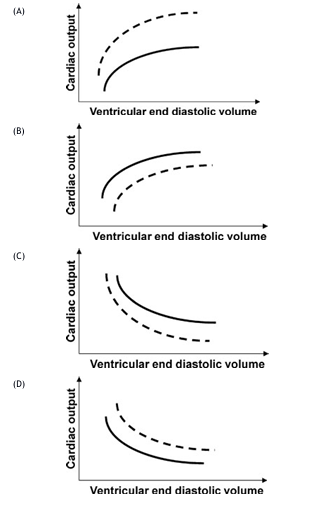
\includegraphics[width=0.7\columnwidth]{FIG/T-16.png}
\caption*{}
\label{T-16}
\end{figure}

\item Match the household insect vectors in \textbf{Column I} with their associated diseases in \textbf{Column II}.

\begin{table}[H]
\centering
\begin{tabular}{ll}
\textbf{Column I} & \textbf{Column II} \\
P. Kissing bug (Hemiptera) & (i) Bubonic plague \\
Q. Sand fly (Diptera) & (ii) Tularemia \\
R. Deer fly (Diptera) & (iii) Chagas disease \\
S. Oriental rat flea (Siphonaptera) & (iv) Kala azar \\
\end{tabular}
\end{table}

\begin{multicols}{2}
\begin{enumerate}[label=(\Alph*)]
\item P-(ii), Q-(iii), R-(i), S-(iv)
\item P-(iii), Q-(iv), R-(ii), S-(i)
\item P-(ii), Q-(iv), R-(iii), S-(i)
\item P-(iii), Q-(iv), R-(ii), S-(i)
\end{enumerate}
\end{multicols}

\item Match the proteins in \textbf{Column I} with the organs in which they are maximally expressed in \textbf{Column II}.

\begin{table}[H]
\centering
\begin{tabular}{ll}
\textbf{Column I} & \textbf{Column II} \\
P. Keratin & (i) Liver \\
Q. Surfactants & (ii) Pancreas \\
R. Pro-carboxypeptidase & (iii) Lung \\
S. Albumin & (iv) Skin \\
\end{tabular}
\end{table}

\begin{multicols}{2}
\begin{enumerate}[label=(\Alph*)]
\item P-(iv), Q-(iii), R-(ii), S-(i)
\item P-(iii), Q-(iv), R-(i), S-(ii)
\item P-(ii), Q-(iii), R-(i), S-(iv)
\item P-(i), Q-(ii), R-(iii), S-(iv)
\end{enumerate}
\end{multicols}

\item The graph below shows the activity of enzyme pepsin in the presence of inhibitors aliphatic alcohols (P) or N-acetyl-L-phenylalanine (Q). Which ONE of the following represents the nature of inhibition by P and Q, respectively?

\begin{figure}[H]
\centering
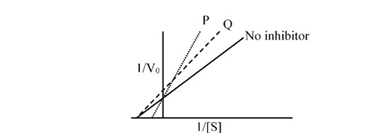
\includegraphics[width=0.7\columnwidth]{FIG/T-19.png}
\caption*{}
\label{T-19}
\end{figure}

\begin{enumerate}[label=(\Alph*)]
\item Non-competitive and competitive
\item Competitive and non-competitive
\item Non-competitive and uncompetitive
\item Competitive and uncompetitive
\end{enumerate}

\item In Drosophila, the red eye phenotype (W) is dominant over the recessive white eye mutant (w). In a mixed population of red and white eye flies of 10,000 individuals, 3,600 flies were white eyed. The percentage of the heterozygous red eye flies in this population is \rule{2.5cm}{0.1pt}.

\end{enumerate}
\newpage
\section*{\centering U : FOOD TECHNOLOGY}

\noindent \textbf{ 1 -- 10 carry one mark each.}

\begin{enumerate}[label=\arabic*.]

\item The enzyme majorly involved in postmortem degradation of muscle proteins is:
\begin{multicols}{2}
\begin{enumerate}[label=(\Alph*)]
\item Trypsin
\item Cathepsin
\item Transglutaminase
\item Pepsin
\end{enumerate}
\end{multicols}

\item Which of the following is the correct pair of essential fatty acids?
\begin{multicols}{2}
\begin{enumerate}[label=(\Alph*)]
\item Oleic acid and Lenoleic acid
\item Lenoleic acid and Linolenic acid
\item Stearic acid and Palmitic acid
\item Linoleic acid and Oleic acid
\end{enumerate}
\end{multicols}

\item Nisin A is produced by
\begin{multicols}{2}
\begin{enumerate}[label=(\Alph*)]
\item Aspergillus niger
\item Saccharomyces cerevisiae
\item Lactobacillus lactis
\item Clostridium perfringens
\end{enumerate}
\end{multicols}

\item Which of the following bacteria will stain purple color after Gram staining?
\begin{multicols}{2}
\begin{enumerate}[label=(\Alph*)]
\item Bacillus subtilis
\item Escherichia coli
\item Pseudomonas aeruginosa
\item Yersinia pestis
\end{enumerate}
\end{multicols}

\item The enzyme system used for removal of glucose from egg white prior to its drying consists of
\begin{multicols}{2}
\begin{enumerate}[label=(\Alph*)]
\item Glucose oxidase and Catalase
\item Glucoamylase and Glucoisomerase
\item Gluconisomerase and Catalase
\item Glucoamylase and Glucose oxidase
\end{enumerate}
\end{multicols}

\item The INCORRECT pair of food borne illness and its causative microorganism is
\begin{multicols}{2}
\begin{enumerate}[label=(\Alph*)]
\item Brucellosis -- Brucella Sp.
\item Peptic ulcers -- Bacillus subtilis
\item Bubonic plague -- Yersinia pestis
\item Q fever -- Coxiella burnetii
\end{enumerate}
\end{multicols}

\item Which of the following is commonly used as a preservative in the tomato sauce?
\begin{multicols}{2}
\begin{enumerate}[label=(\Alph*)]
\item Sodium sulphite
\item Potassium sorbate
\item Potassium sulphite
\item Sodium benzoate
\end{enumerate}
\end{multicols}

\item A fluid with flow behaviour index less than one ($n < 1$) is
\begin{multicols}{2}
\begin{enumerate}[label=(\Alph*)]
\item Dilatant
\item Pseudoplastic
\item Bingham plastic
\item Newtonian
\end{enumerate}
\end{multicols}

\item The velocity of 2.2~$\mu$m diameter fat particles inside a centrifuge, running at 6000~rpm and 20$^\circ$C, is 0.25~mm~s$^{-1}$. The velocity of 1.5~$\mu$m diameter fat particles inside the same centrifuge running at 7500~rpm and same temperature (round off to 2 decimal places) will be \rule{2.5cm}{0.1pt}~mm~s$^{-1}$.

\item The initial population of a bacterial strain increases from $1 \times 10^3$ cells per mL to $1 \times 10^8$ cells per mL in 120 minutes. The generation time for this strain (round off to 2 decimal places) is \rule{2.5cm}{0.1pt}~minutes.

\end{enumerate}

\vspace{0.5cm}

\noindent \textbf{ 11 -- 20 carry two marks each.}

\begin{enumerate}[label=\arabic*.,resume]

\item Match the protein in \textbf{Column I} with its food source in \textbf{Column II}.
\begin{table}[H]
\centering
\begin{tabular}{ll}
\textbf{Column I} & \textbf{Column II} \\
P. Zein & 1. Soybean \\
Q. Gluten & 2. Maize \\
R. Glycinin & 3. Egg \\
S. Ovalbumin & 4. Wheat \\
\end{tabular}
\end{table}

\begin{multicols}{2}
\begin{enumerate}[label=(\Alph*)]
\item P-4, Q-1, R-2, S-3
\item P-4, Q-3, R-1, S-2
\item P-2, Q-3, R-1, S-4
\item P-2, Q-4, R-1, S-3
\end{enumerate}
\end{multicols}

\item Match the carbohydrate in \textbf{Column I} with corresponding enzyme used for its hydrolysis in \textbf{Column II}.
\begin{table}[H]
\centering
\begin{tabular}{ll}
\textbf{Column I} & \textbf{Column II} \\
P. Pectin & 1. Xylanase \\
Q. Lactose & 2. $\beta$-galactosidase \\
R. Hemicellulose & 3. Polygalacturonase \\
S. Inulin & 4. $\beta$-fructofuranosidase \\
\end{tabular}
\end{table}

\begin{multicols}{2}
\begin{enumerate}[label=(\Alph*)]
\item P-3, Q-2, R-1, S-4
\item P-2, Q-4, R-1, S-3
\item P-1, Q-2, R-3, S-4
\item P-4, Q-3, R-1, S-2
\end{enumerate}
\end{multicols}

\item Match the edible oil refining stage in \textbf{Column I} with its purpose in \textbf{Column II}.
\begin{table}[H]
\centering
\begin{tabular}{ll}
\textbf{Column I} & \textbf{Column II} \\
P. Degumming & 1. Separation of triglycerides \\
Q. Neutralization & 2. Removal of pigments \\
R. Bleaching & 3. Removal of phosphatides \\
S. Winterization & 4. Removal of free fatty acids \\
\end{tabular}
\end{table}

\begin{multicols}{2}
\begin{enumerate}[label=(\Alph*)]
\item P-3, Q-1, R-2, S-4
\item P-1, Q-4, R-2, S-3
\item P-4, Q-3, R-1, S-2
\item P-3, Q-4, R-2, S-1
\end{enumerate}
\end{multicols}

\item Match the food material in \textbf{Column I} with its related term in \textbf{Column II}.
\begin{table}[H]
\centering
\begin{tabular}{ll}
\textbf{Column I} & \textbf{Column II} \\
P. Coffee & 1. Wort \\
Q. Cocoa & 2. Must \\
R. Beer & 3. Arabica \\
S. Wine & 4. Theobroma \\
\end{tabular}
\end{table}

\begin{multicols}{2}
\begin{enumerate}[label=(\Alph*)]
\item P-4, Q-2, R-1, S-3
\item P-3, Q-4, R-1, S-2
\item P-3, Q-4, R-2, S-1
\item P-1, Q-3, R-4, S-2
\end{enumerate}
\end{multicols}

\item Match the component/system in \textbf{Column I} with the peeling method for fruits and vegetables in \textbf{Column II}.
\begin{table}[H]
\centering
\begin{tabular}{ll}
\textbf{Column I} & \textbf{Column II} \\
P. Lye solution & 1. Flash peeling \\
Q. Carborundum rollers & 2. Flame peeling \\
R. Pressure vessel & 3. Abrasion peeling \\
S. Conveyor belt & 4. Caustic peeling \\
\end{tabular}
\end{table}

\begin{multicols}{2}
\begin{enumerate}[label=(\Alph*)]
\item P-4, Q-3, R-2, S-1
\item P-3, Q-4, R-1, S-2
\item P-4, Q-3, R-1, S-2
\item P-3, Q-4, R-2, S-1
\end{enumerate}
\end{multicols}

\item Which among the given options correctly explains the nature of the microbial culture represented by lines 1, 2 and 3 in the following figure?
\begin{figure}[H]
\centering
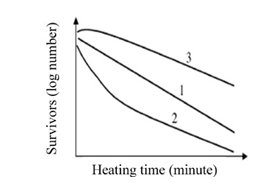
\includegraphics[width=0.7\textwidth]{FIG/U-16.png}
\caption*{}
\label{U-16}
\end{figure}

\begin{enumerate}[label=(\Alph*)]
\item 1. Germination of spores; 2. Homogeneous population; 3. Mixed population of spores and vegetative cells
\item 1. Homogeneous population; 2. Mixed population of heat sensitive and heat resistant microbes; 3. Germination of spores
\item 1. Composite population; 2. Spores activated by short exposure to heat; 3. Thermo sensitive and thermo resistant microbes
\item 1. Mixed population; 2. Microorganisms activated by short exposure to heat; 3. Germination of spores
\end{enumerate}

\item Match the equation/law in \textbf{Column I} with its application in \textbf{Column II}.
\begin{table}[H]
\centering
\begin{tabular}{ll}
\textbf{Column I} & \textbf{Column II} \\
P. Plank's equation & 1. Terminal velocity \\
Q. Arrhenius equation & 2. Freezing time \\
R. Guggenheim-Anderson-de Boer equation & 3. Activation energy \\
S. Stoke's law & 4. Monolayer moisture content \\
\end{tabular}
\end{table}

\begin{multicols}{2}
\begin{enumerate}[label=(\Alph*)]
\item P-1, Q-3, R-4, S-2
\item P-2, Q-3, R-1, S-4
\item P-2, Q-3, R-4, S-1
\item P-4, Q-3, R-1, S-2
\end{enumerate}
\end{multicols}

\item Match the absorber used in modified atmosphere packaging and storage in \textbf{Column I} with the scavenger in \textbf{Column II}.
\begin{table}[H]
\centering
\begin{tabular}{ll}
\textbf{Column I} & \textbf{Column II} \\
P. Oxygen absorber & 1. Calcium chloride \\
Q. Carbon dioxide absorber & 2. Magnesium oxide \\
R. Ethylene absorber & 3. Ferric oxide \\
S. Moisture absorber & 4. Potassium permanganate \\
\end{tabular}
\end{table}

\begin{multicols}{2}
\begin{enumerate}[label=(\Alph*)]
\item P-3, Q-2, R-4, S-1
\item P-1, Q-2, R-4, S-3
\item P-2, Q-3, R-4, S-1
\item P-3, Q-2, R-1, S-4
\end{enumerate}
\end{multicols}

\item During extrusion cooking, food materials are generally subjected to a combination of
\begin{multicols}{2}
\begin{enumerate}[label=(\Alph*)]
\item high shear and low pressure
\item high temperature and high shear
\item low shear and high temperature
\item low shear and low pressure
\end{enumerate}
\end{multicols}

\item An orange juice flowing at $0.80~\mathrm{kg/s}$ enters a counter current double pipe heat exchanger at $20^\circ$C and leaves at $72^\circ$C. Inlet and outlet temperatures of the hot water used as heating medium in the exchanger are $81^\circ$C and $74^\circ$C, respectively. The specific heat of the orange juice is $3.74~\mathrm{kJ/(kg\,K)}$ and overall heat transfer coefficient is $492~\mathrm{W/(m^2\,K)}$. The heat transfer surface area (round off to 2 decimal places) will be \rule{2.5cm}{0.1pt}~$\mathrm{m}^2$.

\end{enumerate}




\end{document}